%!TEX root = ../report.tex

% 
% Architecture
% 
% (2/3pgs)
\section{Architecture}
\label{sec:architecture}

This section describes \emph{ViewZone}, a novel security framework for TrustZone-enabled devices which supports the development of secure sensitive applications, while leveraging Android as the untrusted rich OS, with the particular purpose of displaying privacy sensitive data to the user. This information may take several formats, either being images, pdfs or straight plain text files. This flexibility allows app developers to easily create several basic secure applications such as a secure password managers, sensitive images display (for instance, for military purpose) and sensitive document managers, without ever being at risk of disclosure by a compromised full-featured operating system. To fully demonstrate the concept of \emph{ViewZone}, we develop a sensitive mobile health application for managing personal health records. The following subsections describe the underlying \emph{ViewZone} system architecture and the purposed \ac{PHR} application.

%% ==== SYSTEM ====
\subsection{ViewZone}

\emph{ViewZone} must maintain a small trusted computing base in order to guarantee a secure foundation for sensitive applications. This means only the strictly necessary features for practical applications to work must be supported, and even these features must be built with intelligent and conservative development strategies. Moreover, \emph{ViewZone} must allow for an integrated environment with Android to provide a transparent isolated security environment for these sensitive applications without compromising the system's usability. To support the described features this project must fulfil the goals of assuring the necessary security policies such as confidentiality, integrity and authenticity of data stored in the untrusted world, must support trusted user interfaces and be developer friendly, which is allow for easy development of simple secure applications such as those described above. The following paragraphs describe how these goals will be supported in \emph{ViewZone}.

\paragraph{\textbf{Secure Storage}}

In order to bypass the physical limitations of storage in the secure world domain a different strategy must be implemented to support secure storage of large files. Inspired by the work which culminated on the development of DroidVault~\cite{li2014droidvault}, secure storage is possible by enabling large files to be stored in the untrusted domain. To achieve this goal \emph{ViewZone} must implement, similarly to what is done in DroidVault, a \ac{DPM}, which is the secure module for data operations. A file can be created inside \emph{ViewZone}, or downloaded from a remote server, and encrypted with a key generated in the secure side, or known by it. This way, sensitive data is encrypted before leaving \emph{ViewZone} and is never disclosed to the Android OS. Moreover, \ac{DPM} can verify if a client application running in Android (front-end of a \emph{ViewZone} trusted application) is the owner of the encrypted data, if it is then the \ac{DPM} is responsible for loading the corresponding file in the secure world domain so it can be securely managed by the trusted application. The \ac{DPM} assures the confidentiality and integrity of sensitive data in \emph{ViewZone} and allows for large files to be securely stored in the untrusted domain of a TrustZone-enabled mobile device.

\paragraph{\textbf{Secure World-Switching}}

A big limitation of some systems described in section~\ref{sec:relatedWork} is world-switching based on software interrupts, which allow denial-of-service attacks by a malicious rich operating system that may sabotage inter-world calls responsible for the world switch. To mitigate such attacks, hardware interrupts responsible for the world-switching mechanism were implemented by the authors of TrustOTP~\cite{sun2015trustotp} and TrustDump~\cite{sun2015reliable} in these systems. \ac{NMI} are hardware interrupts that cannot be ignored by standard interrupt masking techniques, typically used to signal attention for non-recoverable hardware errors, can be used in order to feature secure world switches between the normal and secure world domains. With these interrupts the user can be guaranteed of an inter-world switch and that the operations dependent of this world switch are authentic, this is because the secure domain is non-reentrant, meaning that after the system enters the secure domain, the system will switch back to the rich OS only when \emph{ViewZone} explicitly triggers the switch.

\paragraph{\textbf{Trusted User Interface}}

Most trusted execution environments support the execution of code on the secure side, thus supporting some basic secure services. But without a user interface support for user-machine interaction, these systems limit greatly the potential for practical trusted applications. Because user interfaces play a big role in improving app usability, trusted applications must support trusted user interfaces to be useful and so the data from and to the trusted application cannot be eavesdropped by the rich operating system. To achieve this a secure display controller must be implemented to securely copy the image from a secure framebuffer to the display device, where the framebuffer stores the image to be displayed. By having different framebuffers for the secure and normal domains, \emph{ViewZone} can prevent potential data leakage, as the secure framebuffer is reserved for use in the secure world. Moreover, because usually resources such as the video card and display screen are shared by both domains, the reliable display controller must be able to correctly program both resources. On the other hand, to support trusted input from the user, a self-contained secure screen driver must be included in the secure world domain. With these mechanism there is a guarantee that the information displayed to the user and the information given as input to the system is authentic.

\paragraph{\textbf{Developer Friendly}}

Trusted execution environments already present some developer friendly strategies to easily allow new trusted application development. This is generally done by supporting applications built using GlobalPlatform's APIs. But to feature more complex mechanisms, such as trusted user interfaces, some trusted applications have to manage low level resources, such as the graphical framebuffer, directly. This highly increases the complexity of developing trusted applications and is unnecessary to implement specifically for every app as most of them require such mechanims to be useful. For this reason, \emph{ViewZone} implements an API for an easy development of trusted applications which leverage resources such as the graphical framebuffer (for trusted UI), secure shared memory and inter-world communication, and secure storage.

% DIGO QUE ISTO EXISTE MAS NAO EXPLICO COMO FUNCIONA

% ARQUITECTURA
\begin{figure}[t!]
	\centering
	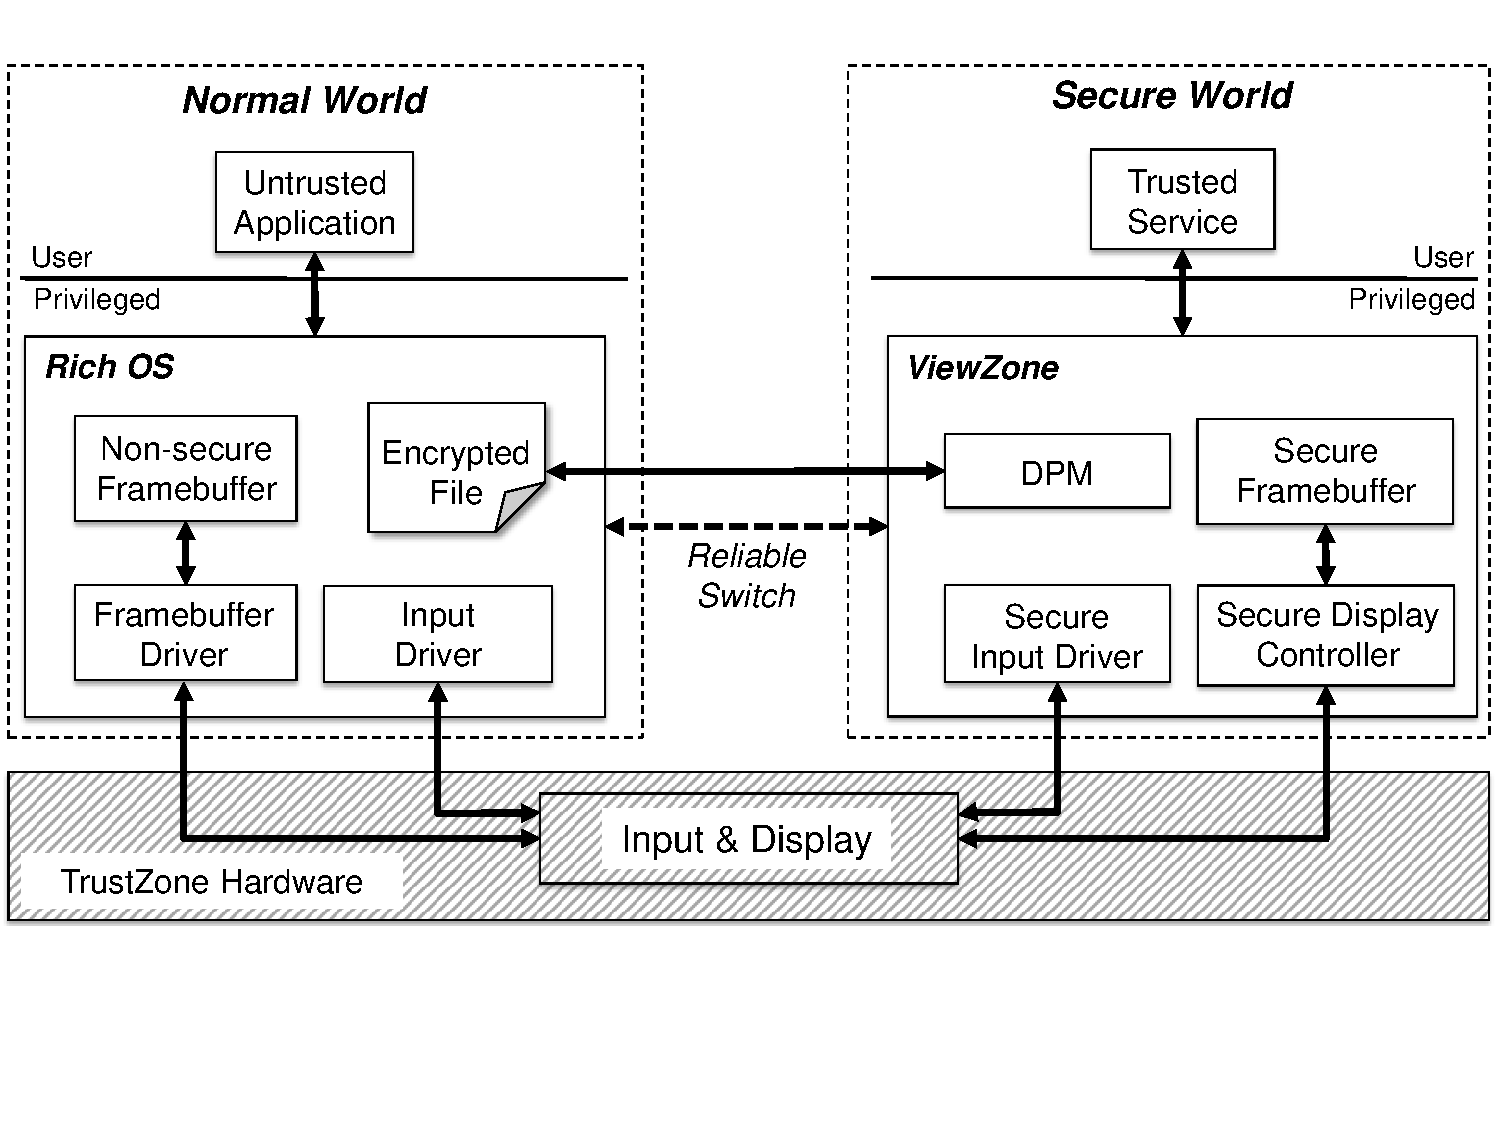
\includegraphics[width=0.9\textwidth]{img/viewzone_architecture.pdf}
	\caption{ViewZone's Architecture}
	\label{fig:viewzone_architecture}
\end{figure}

\paragraph{\textbf{Architecture}} Figure~\ref{fig:viewzone_architecture} combines all the components, techniques and mechanisms described above into \emph{ViewZone}'s architecture. An untrusted applications running in the rich OS works as a front-end for the trusted service in the secure domain. This untrusted application loads the encrypted sensitive file, whose content is only accessible by the secure world, into a shared memory region. This shared memory region allows the \ac{DPM} to securely copy the encrypted file to an isolated secure memory region so it can be decrypted and later displayed to the user. The \ac{DPM} looks into the shared memory region only when the reliable switch is triggered by the secure \ac{NMI} hardware interrupt, thus assuring the subsequent operations are executed by the secure side, meaning the content displayed is authentic. Once the \ac{DPM} has access to the sensitive file content, the secure display controller copies the non-secure framebuffer to the secure framebuffer and the content of the sensitive file can be integrated with that of the original framebuffer, thus giving the impression of integrated user interface between the untrusted and secure domains. This way, the trusted service can display content as it would be displayed by the original rich OS interface. The input is also controlled by the secure world by using the specific input driver in the trusted domain. When another \ac{NMI} interrupt is triggered, the \ac{DPM} encrypts the file again and returns it to the shared memory region where it was first loaded by the untrusted application, thus allowing the trusted service to edit the file, which will then be stored in the untrusted domain.